%%%%%%%%%%%%%%%%%%%%%%%%%%%%%%%%%%%%%%%%%
% Dreuw & Deselaer's Poster
% LaTeX Template
% Version 1.0 (11/04/13)
%
% Created by:
% Philippe Dreuw and Thomas Deselaers
% http://www-i6.informatik.rwth-aachen.de/~dreuw/latexbeamerposter.php
%
% This template has been downloaded from:
% http://www.LaTeXTemplates.com
%
% License:
% CC BY-NC-SA 3.0 (http://creativecommons.org/licenses/by-nc-sa/3.0/)
%
%%%%%%%%%%%%%%%%%%%%%%%%%%%%%%%%%%%%%%%%%

%----------------------------------------------------------------------------------------
%	PACKAGES AND OTHER DOCUMENT CONFIGURATIONS
%----------------------------------------------------------------------------------------

\documentclass[final,hyperref={pdfpagelabels=false}]{beamer}

\usepackage[orientation=portrait,size=a0,scale=1.25]{beamerposter} % Use the beamerposter package for laying out the poster with a portrait orientation and an a0 paper size

\usetheme{I6pd2} % Use the I6pd2 theme supplied with this template

\usepackage[english]{babel} % English language/hyphenation

\usepackage{amsmath,amsthm,amssymb,latexsym} % For including math equations, theorems, symbols, etc

%\usepackage{times}\usefonttheme{professionalfonts}  % Uncomment to use Times as the main font
%\usefonttheme[onlymath]{serif} % Uncomment to use a Serif font within math environments

\boldmath % Use bold for everything within the math environment

\usepackage{booktabs} % Top and bottom rules for tables

\graphicspath{{figures/}} % Location of the graphics files

\usecaptiontemplate{\small\structure{\insertcaptionname~\insertcaptionnumber: }\insertcaption} % A fix for figure numbering

%--------------------------------
% CUSTOM COMMANDS ETC.
%---------------------------------
\renewcommand{\Re}{\operatorname{Re}}
\renewcommand{\Im}{\operatorname{Im}}
\usepackage{braket}
\newcommand{\mean}[1]{\langle #1 \rangle}


%----------------------------------------------------------------------------------------
%	TITLE SECTION 
%----------------------------------------------------------------------------------------

\title{\huge An Alternative to Contextuality} % Poster title

\author{Atul Singh Arora \\ \small supervisor: Prof. Arvind} % Author(s)

%\institute{{\small Quantum Computation \& Quantum Information (QCQI) Group,} Indian Institute of Science Education \& Research (IISER), Mohali} % Institution(s)
\institute{Indian Institute of Science Education \& Research (IISER), Mohali} % Institution(s)

%----------------------------------------------------------------------------------------
%	FOOTER TEXT
%----------------------------------------------------------------------------------------

\newcommand{\leftfoot}{}  %http://www.LaTeXTemplates.com} % Left footer text

\newcommand{\rightfoot}{} %john@smith.com} % Right footer text

%----------------------------------------------------------------------------------------

\begin{document}

\addtobeamertemplate{block
  end}{}{\vspace*{2ex}} % White space under blocks

\begin{frame}[t] % The whole poster is enclosed in one beamer frame

  \begin{columns}[c] % The whole poster consists of two major columns, each of which can be subdivided further with another \begin{columns} block - the [t] argument aligns each column's content to the top

    \begin{column}{.01\textwidth}\end{column} % Empty spacer column
    \begin{column}{.32\textwidth} % The first column

      % ----------------------------------------------------------------------------------------
      % BACKGROUND
      % ----------------------------------------------------------------------------------------
      \begin{block}{Background}
        \begin{columns}
          \begin{column}{0.7\textwidth}
            \begin{itemize}
            \item Einstein: `locality' $\implies$ Quantum Mechanics (QM) is incomplete. 

            \item Bell: `locality'  $\implies \mean {\hat B} \le 2$; For some $\ket{\psi}$, QM $\implies \mean{\hat B} = 2\sqrt 2$. Verified experimentally (without loop holes in 2015)

            \item Comment: At roughly the same time, various physicists had produced proofs of the claim that one can't complete QM satisfactorily, that a sensible complete `hidden variable' (HV) description of nature was impossible. 

            \item Bohmian Mechanics (BM): a HV description, that (i) `completes' QM in a simple, clear, precise but non-local manner, and (ii) is deterministic.

            \item Defn: \emph{Deterministic} $\equiv$ If in principle, the outcome of measuring each observable is predictable, given the HVs. %Probabilities enter the description because of our ignorance and is not intrinsic to nature.

            \item Comment: Bell's inequality requires entanglement in some form, to prove Einstein's notion of locality incorrect. Recently, another peculiar feature of QM has been identified, namely contextuality. 

            \item Impl Defn: \emph{Context} $\equiv$ If $[A,B]=0$ and $[A,C]=0$ but $[B,C]\neq 0$, then possible contexts are {A}, {A and B} or {A and C}.

            \item Defn: \emph{Non-contextual} $\equiv$ Value an operator takes, depends only on the state (including `hidden variables) and the choice of the operator $A$ (not it's context).

            \item Defn: \emph{Contextual} $\equiv$ Value an operator takes, depends on it's context.

            \item Comment: This notion arises, atleast in certain explicit constructions, where one is unable to assign values to operators, consistent with predictions of QM.

            \item Aim: Understand how a deterministic theory can be consistent with the notion of contextuality.
            \end{itemize}
          \end{column}

          \begin{column}{0.3\textwidth}
            \begin{figure}
              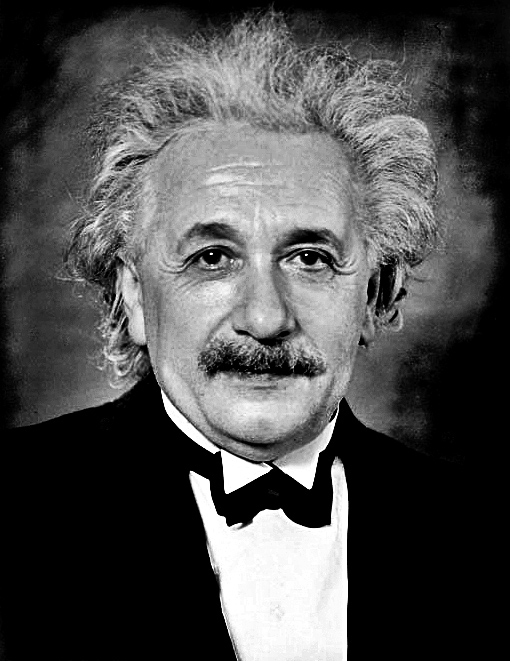
\includegraphics[width=0.8\linewidth]{einstein}
              \caption{A. Einstein}
            \end{figure}
            \begin{figure}
              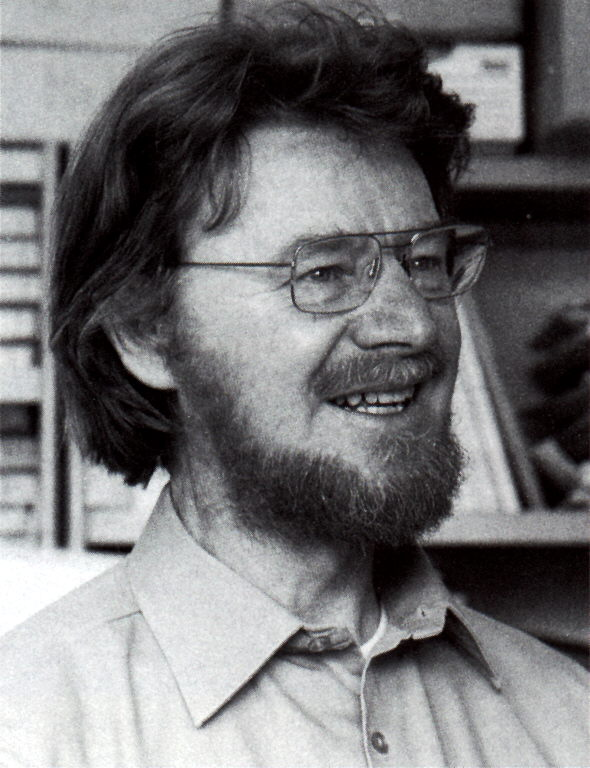
\includegraphics[width=0.8\linewidth]{bell}
              \caption{J. Bell}
            \end{figure}
            \begin{figure}
              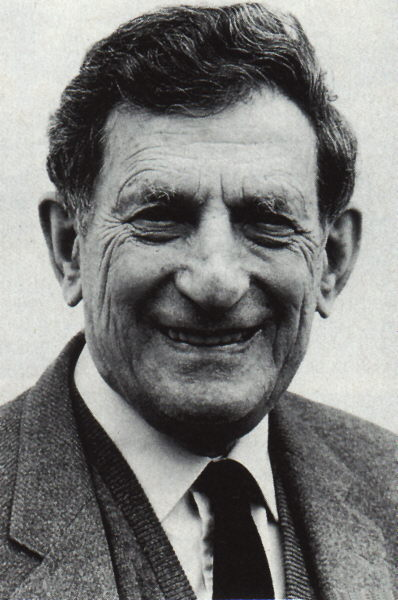
\includegraphics[width=0.8\linewidth]{bohm}
              \caption{D. Bohm}
            \end{figure}
            \begin{figure}
              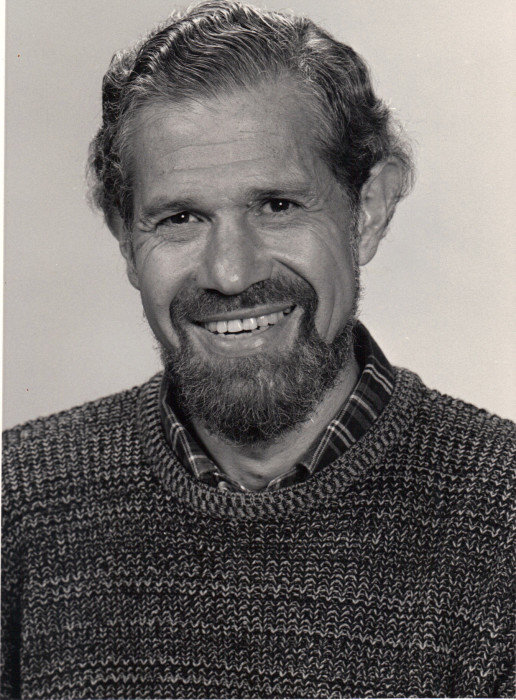
\includegraphics[width=0.8\linewidth]{kochen}
              \caption{S. B. Kochen}
            \end{figure}

          \end{column}
      \end{columns}
        % Einstein was able to demonstrate that if one assumes `locality', then one can show that quantum mechanics must be incomplete. Later Bell showed that one can test Einstein's notion of `locality' by arriving at an inequality which any `local' theory must satisfy, while Quantum Mechanics (QM) he showed, could violate. Experimentally, it has been conclusively shown, that the said notion of `locality' must be given up.

        % At roughly the same time, various physicists had produced proofs of the claim that one can't complete QM satisfactorily, that a sensible complete `hidden variable' (HV) description of nature was impossible. de Broglie and Bohm were able to arrive at precisely such a HV description, known as Bohmian Mechanics (BM). This description `completes' QM in an simple, clear, precise but non-local manner. BM is deterministic, that is it can predict in principle, the outcome of measuring each observable, given we know the HVs. Probabilities enter the description because of our ignorance and is not intrinsic to nature.

        % Bell's inequality requires entanglement in some form, to prove Einstein's notion of locality incorrect. Recently, another peculiar feature of QM has been identified, namely contextuality. This notion arises, atleast in certain explicit constructions, where one is unable to assign values to operators, consistent with predictions of QM. Thus one concludes that the value an operator takes, must depend on the complete set of compatible observables being measured.

        % The present work was motivated by an attempt to understand how a deterministic theory can be consistent with the notion of contextuality.
      \end{block}

      % ----------------------------------------------------------------------------------------
      % INTRODUCTION
      % ----------------------------------------------------------------------------------------
      
      \begin{block}{Overview}

            \begin{figure}
              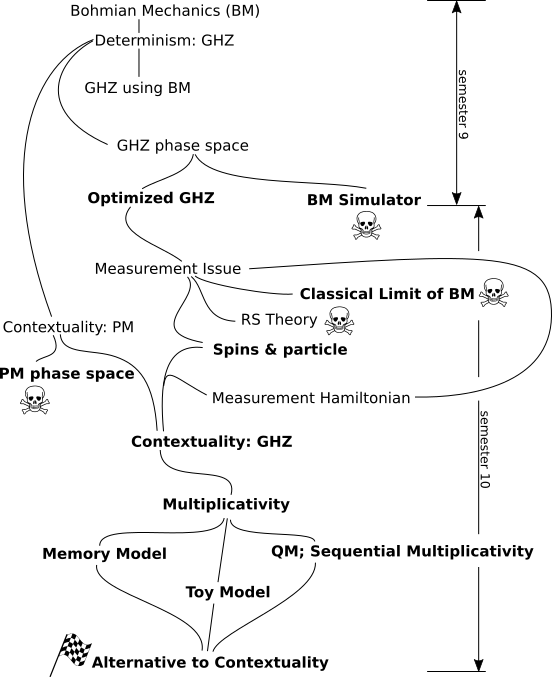
\includegraphics[width=0.99\linewidth]{flow.png}
              \caption{Exploration flow: Boldface titles represent new results}
            \end{figure}
        

        % To investigate the aforesaid issue, in the previous semester, in addition to learning BM, I explored how the GHZ test (a test of determinism) is explained using BM. The lesson learnt was that there's no direct contradiction, because BM never assigned values to spins. However, since QM treats phase space variables, in essentially the same way as spins, it was found that the GHZ test can be extended to phase space also. BM asserts that phase space variables have pre-defined values, and here, the QM test claim that phase space variables can't have pre-defined values, is in direct contradiction with BM. It was concluded that this situation will edify the mysterious co-existence of the two notions.
        
        % With the problem narrowed, tools required to solve it were developed. Since it is known that obtaining BM trajectories analytically is not trivial, a `proof of principle' simulator was written and tested. In addition, it was noted that the phase-space GHZ test would require optimization, since it involved un-normalized states, which are impossible to simulate directly. Considerable attempts were made at first optimizing the test, all of which failed. In the following semester however, an optimization operator was constructed, which was able to yield the GHZ situation, for finite states. The cost that had to be paid, was that the observables had to be made functions of $q$ and $p$ both, instead of only $p$ (or $q$) as was the case earlier. Recall that BM only specifies values of functions of $q$ and $p$ seperately. Thus the theoretical basis of measurements in BM was studied in further detail. Infact, in the process, it was found, in an attempt at obtaining the classical limit of measurements, that obtaining classical mechanics (CM) from BM, is infact not as simple as it appears from taking $\hbar \to 0$.

        % Newer difficulties were faced upon realizing that the value of $p$ that a particle has in BM, is not necessarily the value one observes upon measurement. This is explained quite satisfactorily in the BM framework, by showing that the process of measurement leads to transfer of momentum. One direction which was suggested by Prof. Arvind, was a `maximally complete' description of QM by Roy Singh (RS). In this formalism, both $q$ and $p$ have predefined values consistent with the values obtained after measurement. The issue however prevailed, since the generalized GHZ test required measurement of functions of $q$ and $p$ together, which again, weren't easy to evaluate from the RS description.

        % It was also realized that in addition to the measurement issues, there did not seem any concievable way of explaining the contextuality tests using BM. Since values assigned to compatible operators, must be consistent with the values assigned to any function of these operators, it follows from the construction of these tests, that one can't assign values (therefore predict) even in principle. With the GHZ, this wasn't as profound a problem, because the operators involved didn't have to commute and thus value assigned to a product of two non-commuting observables, was not required to be a product of those assigned to the constituent operators.

        % To escelate the contextuality test, it was generalized to phase space and attempts were made to optimize it. Parallelly, attempts were also made at understanding how spins are measured using BM, and alternate proofs of the fact that within BM, spins can't be associated with particles, were obtained. It was finally realized that one needn't extend tests to phase space, to arrive at an apparent contradiction between QM and BM. From consistency requirements of both, a new property, termed by us `non-multiplicativity' was speculated. Finally, a toy-model was constructed, which is non-contextual and still violates the PM inequality. 

        % In summary then, we have shown that we can have a deterministic view of the world, with `non-multiplicativity' as the non-classical feature, as opposed to contextuality; we have identified an alternative to contextuality.
      \end{block}

\end{column}
\begin{column}{.01\textwidth}\end{column} % Empty spacer column
\begin{column}{.32\textwidth} % The first column


  % ----------------------------------------------------------------------------------------
  % Contextuality
  % ----------------------------------------------------------------------------------------

  \begin{block}{Contextuality - PM Test}
    Defn: \emph{Compatible operators} $\equiv$ Two observables $A$ and $B$ are mutually compatible if the result of measuring $A$ doesn't depend on whether $B$ is measured (before, after, simultaneously or not measured at all). TODO: Update this definition.

    Defn: \emph{Non-contextually Deterministic} $\equiv$ If we restrict ourselves to hidden variable models that assert that $A$ and $B$ have predefined values, irrespective of which compatible observable is measured, then such a theory would be termed ``non-contextual'' and deterministic. 

    Result: Kochen-Specker proved that such theories, viz. non-contextual deterministic theories are inconsistent with QM. Mermin and Peres showed this for a four-level system. 

    Proof: Consider the following operators. 
    \[
    A_{ij} \doteq \left[
    \begin{array}{ccc}
       \sigma_z\otimes \mathbb I &  \mathbb I \otimes \sigma_z & \sigma_z\otimes \sigma_ z \\
       \mathbb I \otimes \sigma_x &  \sigma_x \otimes \mathbb I & \sigma_x\otimes \sigma_x \\
       \sigma_z \otimes \sigma_x &  \sigma_x \otimes \sigma_z & \sigma_y\otimes \sigma_y
    \end{array} \right]
    \]

    % \begin{array}{ccc}
    %   A_{11} = \sigma_z\otimes \mathbb I & A_{12} = \mathbb I \otimes \sigma_z & A_{13}=\sigma_z\otimes \sigma_ z \\
    %   A_{21} = \mathbb I \otimes \sigma_x & A_{22} = \sigma_x \otimes \mathbb I & A_{23}=\sigma_x\otimes \sigma_x \\
    %   A_{31} = \sigma_z \otimes \sigma_x & A_{32} = \sigma_x \otimes \sigma_z & A_{33}=\sigma_y\otimes \sigma_y
    % \end{array}

    Note that operators along a given row (column) commute. 
    
    \begin{align}
      R_i\equiv \prod_j A_{ij} & = \mathbb{I} \\
      C_j\equiv \prod_i A_{ij} & = 
                                 \begin{cases} 
                                   +\mathbb{I} &  (j\neq 3)\\
                                   -\mathbb{I} &  (j=3)
                                 \end{cases} 
    \end{align}
It entails that $\prod_{k=1,2,3}R_kC_k= -\mathbb{I}$, whereas non-contextual models would yield +1.

To facilitate experimental validation, it has been shown that non-contextual models satisfy Eq. \ref{eq:pm}, while QM yields $\mean{\chi_{PM}}=6$.
  \begin{equation}
    \mean{\chi_{PM}} = \mean{R_1} + \mean{R_2} + \mean{R_3} + \mean{C_1} + \mean{C_2} - \mean{C_3} \le 4
    \label{eq:pm}
  \end{equation}

  % \begin{figure}
  %   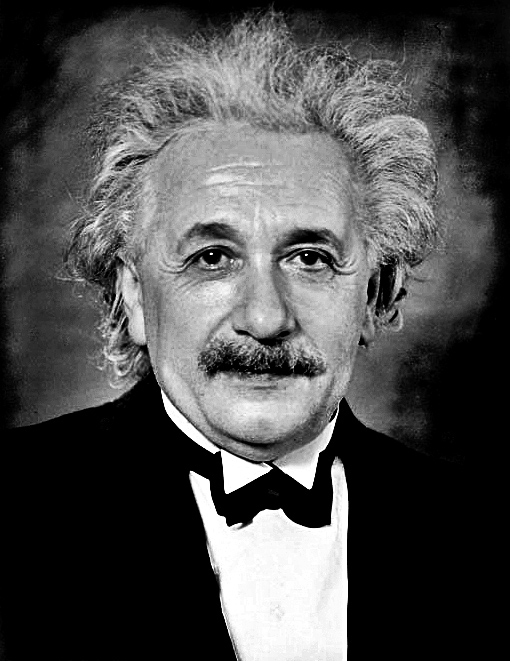
\includegraphics[width=0.8\linewidth]{einstein}
  %   \caption{A. Einstein}
  % \end{figure}

%This also holds for a given column and thus these are compatible. Also note that the measurement product along any row ($R_K$) or column ($C_k$) is 1, except for column three; $C_3=-1$. Thus, QM predicts $\prod_{k=1,2,3}R_kC_k=-1$, in contrast to non-contextual models. Since no experiment yields ideal results, an inequality must be constructed. It has been shown that all non-contextual theories must satisfy $\mean{\chi_{KS}} = \mean{R_1} + \mean{R_2} + \mean{R_3} + \mean{C_1} + \mean{C_2} - \mean{C_3} \le 4$. QM yields $\mean{\chi_{KS}}=6$. 

  \end{block}

  % ----------------------------------------------------------------------------------------
  % Memory Model
  % ----------------------------------------------------------------------------------------

  \begin{block}{Contextuality - Memory Model}
    Initial: The assignment is as given in Mat \ref{eq:allPlus}. 

    Remark: The system is assumed to be capable of remembering the last three observables that were measured. 

    Algorithm: Upon measurement of an observable, (i) yield the value as saved in the matrix, (ii) append the observable in the 3 element memory and (iii) update the matrix, once the context (set of commuting observables) is known, to satisfy the PM requirements.
    \begin{equation}\label{eq:allPlus}
\left[
    \begin{array}{ccc}
      1 & 1 & 1 \\
      1 & 1 & 1 \\
      1 & 1 & 1
    \end{array} 
\right]
    \end{equation}

    For example:
    \[
    \begin{array}{c|ccc}
      \text{Operator} & \text{Updated Array} & \text{New Assignment} & \text{Value}\\
      \hat {A}_{33} & \{*,*,\hat{A}_{33}\} & \text{Mat \ref{eq:allPlus}} & 1\\
      \hat {A}_{23} & \{*,\hat{A}_{33},\hat{A}_{23}\} & \text{Mat \ref{eq:oneMinus}} & 1\\
      \hat {A}_{13} & \{\hat{A}_{33},\hat{A}_{23},\hat {A}_{13}\} & \text{Mat \ref{eq:oneMinus}} & -1
    \end{array}
    \]

    \begin{equation}\label{eq:oneMinus}
      \left[
    \begin{array}{ccc}
      1 & 1 & -1 \\
      1 & 1 & 1 \\
      1 & 1 & 1
    \end{array} 
    \right]
    \end{equation}

    Result: $C_3=-1$ as required.

  \end{block}

  % ----------------------------------------------------------------------------------------

\end{column}
\begin{column}{.01\textwidth}\end{column} % Empty spacer column
\begin{column}{.32\textwidth} % The first column

  % ----------------------------------------------------------------------------------------
  % Multiplicativity
  % ----------------------------------------------------------------------------------------

  \begin{block}{Multiplicativity}
    \begin{itemize}
      \item Defn: \emph{Multiplicativity} $\equiv$ For compatible operators $\hat{B_i}$, a model is multiplicative iff 
        \begin{align} f(m_1(\hat{B}_1),m_1(\hat{B}_2),&\dots,m_1(\hat{B}_n)) = \\
          &m_1(f(\hat{B}_1,\hat{B}_2,\dots,\hat{B}_n),
        \end{align}
        where $m_j(\hat *)$ represents the assigned value of the operator, and $j$ encodes the sequence of measurement. Note that this is an ontological statement and can't be experimentally tested.

      \item Defn: \emph{Sequential Multiplicativity} $\equiv$ For compatible operators $\hat{B_i}$, a model is sequentially multiplicative iff 
        \begin{align} f(m_{k_1}(\hat{B}_1),m_{k_2}(\hat{B}_2),&\dots,m_{k_n}(\hat{B}_n)) = \\
          &m_1(f(\hat{B}_1,\hat{B}_2,\dots,\hat{B}_n),
        \end{align}
        where $\mathbf k \equiv (k_1,k_2,\dots,k_n) \in ((1,2,\dots,n)$ + all possible permutations $)$, $m_j(\hat *)$ represents the assigned value of the operator, and $j$ encodes the sequence of measurement.

      \item Example: $\hat B_1 = \hat {\sigma} _x \otimes \hat {\sigma}_y$, $\hat B_2 = \hat {\sigma} _y \otimes \hat {\sigma}_x$ so that $\hat C = \hat B_1 \hat B_2 = \hat \sigma _z \otimes \hat \sigma _z$. $\ket {\psi}=\ket{00}$, so that $m_1(\hat C)=1$, while $m_1(\hat B_i)=\pm 1$. If say $m_1(\hat B_1)=-1$, then ${\psi} \to \text{(figure this)}$ so that entails $m_2(\hat B_2)=-1$ as well, consistent with $m_1(\hat C)=m_1(\hat B_1)m_2(\hat B_2)$.

      \item Result: Quantum Mechanics is sequentially multiplicative.

    \end{itemize}
     
  \end{block}

  % ------------------------------------------------
  % The Toy Model
  % ------------------------------------------------
  \begin{block}{The Toy Model}
    \begin{itemize}
      \item Initial: $\ket {\psi}$; 
      \item `hidden variable': Choose $c=+1$ for heads, $c=-1$ for tails, after a coin toss
      \item Predictions/Assignments: For an operator $\hat{p}'\in\{\hat{A}_{ij},\hat{R}_{i},$ + their products such as $\hat{C}_{j}\,(\forall\,i,j)\}$  check if $\exists$ a $\lambda$, s.t. $\hat{p}'\left|\psi\right\rangle =\lambda\left|\psi\right\rangle$. If $\exists$ a $\lambda$, then assign $\lambda$ as the value. Else, assign c.
      \item Update: Say $\hat{p}$ was observed. If $\hat{p}$ is s.t. $\hat{p}\left|\psi\right\rangle =\lambda\left|\psi\right\rangle$, then leave the state unchanged. Else, find $\left|p_{\pm}\right\rangle$   (eigenkets of $\hat{p}$), s.t. $\hat{p}\left|p_{\pm}\right\rangle =\pm\left|p_{\pm}\right\rangle$ and update the state $\left|\psi\right\rangle \to\left|p_{c}\right\rangle$. 
    \end{itemize}

  \end{block}
  \begin{block}{The Toy Model | Example}
    {\small
    \begin{equation}
      \begin{array}{c|ccc}
        \text{Iteration} & i=1 & i=2 & i=3\\
        \left|\psi_{\text{init}}\right\rangle  & \left|00\right\rangle  & \left|00\right\rangle  & \frac{\left|00\right\rangle +\left|11\right\rangle }{\sqrt{2}}\\
        \text{HV/Toss} & c=-1 & c=-1 & c=+1\\
        \\
        \text{Predictions} & m_{1}(\hat{A}_{ij})\doteq\left[\begin{array}{ccc}
                                                              -1 & -1 & -1\\
                                                              -1 & -1 & -1\\
                                                              -1 & -1 & +1
                                                            \end{array}\right] & m_{2}(\hat{A}_{ij})\doteq\left[\begin{array}{ccc}
                                                                                                                  -1 & -1 & -1\\
                                                                                                                  -1 & -1 & -1\\
                                                                                                                  -1 & -1 & +1
                                                                                                                \end{array}\right] & m_{3}(\hat{A}_{ij})\doteq\left[\begin{array}{ccc}
                                                                                                                                                                      +1 & +1 & +1\\
                                                                                                                                                                      +1 & +1 & -1\\
                                                                                                                                                                      +1 & +1 & +1
                                                                                                                                                                    \end{array}\right]\\
        \text{(Assignments)}\\
                         & m_{1}(\hat{R}_{i}),m_{1}(\hat{C}_{j})=+1\,(j\neq3) & m_{2}(\hat{R}_{i}),m_{2}(\hat{C}_{j})=+1\,(j\neq3) & m_{3}(\hat{R}_{i}),m_{3}(\hat{C}_{j})=+1\,(j\neq3)\\
                         & m_{1}(\hat{C}_{3})=-1 & m_{2}(\hat{C}_{3})=-1 & m_{3}(\hat{C}_{3})=-1\\
        \text{Operator}\\
        \text{Measured} & \hat{A}_{13}=\hat{\sigma}_{z}\otimes\hat{\sigma}_{z};m_{1}(\hat{A}_{13})=+1 & \quad\quad\hat{A}_{23}=\hat{\sigma}_{y}\otimes\hat{\sigma}_{y};m_{2}(\hat{A}_{23})=-1\quad\quad & \hat{A}_{33}=\hat{\sigma}_{x}\otimes\hat{\sigma}_{x};m_{3}(\hat{A}_{33})=+1\\
        \\
        \left|\psi_{\text{final}}\right\rangle  & \left|00\right\rangle  & \frac{\left|00\right\rangle +\left|11\right\rangle }{\sqrt{2}} & \frac{\left|00\right\rangle +\left|11\right\rangle }{\sqrt{2}}
      \end{array}
    \end{equation}}
  \end{block}

  % ----------------------------------------------------------------------------------------
  % CONCLUSION
  % ----------------------------------------------------------------------------------------

  \begin{block}{Conclusion}


  \end{block}

  % ----------------------------------------------------------------------------------------
  % REFERENCES
  % ----------------------------------------------------------------------------------------

  \begin{block}{References}
        
    \nocite{*} % Insert publications even if they are not cited in the poster
    \small{\bibliographystyle{unsrt} \bibliography{sample}}

  \end{block}

  % ----------------------------------------------------------------------------------------
  % ACKNOWLEDGEMENTS
  % ----------------------------------------------------------------------------------------

  \begin{block}{Acknowledgments}


  \end{block}

  % ----------------------------------------------------------------------------------------
  % CONTACT INFORMATION
  % ----------------------------------------------------------------------------------------

  \setbeamercolor{block
    title}{fg=black,bg=orange!70} % Change the block title color

  \begin{block}{Contact Information}

    \begin{itemize}
    %\item Web:      \href{http://www.university.edu/smithlab}{http://www.university.edu/smithlab}
    \item Email: \href{mailto:ms11003@iisermohali.ac.in}{ms11003@iisermohali.ac.in}
    \item Email: \href{mailto:to.AtulArora@gmail.com}{to.AtulArora@gmail.com}
    \item Phone: +91 8699 413350
    \end{itemize}

  \end{block}

  % ----------------------------------------------------------------------------------------

\end{column} % End of the second column

\begin{column}{.015\textwidth}\end{column} % Empty spacer column

\end{columns} % End of all the columns in the poster


\end{frame} % End of the enclosing frame

\end{document}